% ******************************************************** %
%              TEMPLATE DE INFORME ORGA2 v0.1              %
% ******************************************************** %
% ******************************************************** %
%                                                          %
% ALGUNOS PAQUETES REQUERIDOS (EN UBUNTU):                 %
% ========================================
%                                                          %
% texlive-latex-base                                       %
% texlive-latex-recommended                                %
% texlive-fonts-recommended                                %
% texlive-latex-extra?                                     %
% texlive-lang-spanish (en ubuntu 13.10)                   %
% ******************************************************** %


\documentclass[a4paper]{article}
\usepackage[spanish]{babel}
\usepackage[utf8]{inputenc}
\usepackage{charter}   % tipografia
\usepackage{graphicx}
%\usepackage{makeidx}
\usepackage{paralist} %itemize inline

%\usepackage{float}
%\usepackage{amsmath, amsthm, amssymb}
%\usepackage{amsfonts}
%\usepackage{sectsty}
%\usepackage{charter}
%\usepackage{wrapfig}
%\usepackage{listings}
%\lstset{language=C}

% \setcounter{secnumdepth}{2}
\usepackage{underscore}
\usepackage{caratula}
\usepackage{url}


% ********************************************************* %
% ~~~~~~~~              Code snippets             ~~~~~~~~~ %
% ********************************************************* %

\usepackage{color} % para snipets de codigo coloreados
\usepackage{fancybox}  % para el sbox de los snipets de codigo

\definecolor{litegrey}{gray}{0.94}

\newenvironment{codesnippet}{%
	\begin{Sbox}\begin{minipage}{\textwidth}\sffamily\small}%
	{\end{minipage}\end{Sbox}%
		\begin{center}%
		\vspace{-0.4cm}\colorbox{litegrey}{\TheSbox}\end{center}\vspace{0.3cm}}



% ********************************************************* %
% ~~~~~~~~         Formato de las páginas         ~~~~~~~~~ %
% ********************************************************* %

\usepackage{fancyhdr}
\pagestyle{fancy}

%\renewcommand{\chaptermark}[1]{\markboth{#1}{}}
\renewcommand{\sectionmark}[1]{\markright{\thesection\ - #1}}

\fancyhf{}

\fancyhead[LO]{Sección \rightmark} % \thesection\ 
\fancyfoot[LO]{\small{Nombre Apellido, Nombre Apellido, Nombre Apellido}}
\fancyfoot[RO]{\thepage}
\renewcommand{\headrulewidth}{0.5pt}
\renewcommand{\footrulewidth}{0.5pt}
\setlength{\hoffset}{-0.8in}
\setlength{\textwidth}{16cm}
%\setlength{\hoffset}{-1.1cm}
%\setlength{\textwidth}{16cm}
\setlength{\headsep}{0.5cm}
\setlength{\textheight}{25cm}
\setlength{\voffset}{-0.7in}
\setlength{\headwidth}{\textwidth}
\setlength{\headheight}{13.1pt}

\renewcommand{\baselinestretch}{1.1}  % line spacing

% ******************************************************** %


\begin{document}


\thispagestyle{empty}
\materia{Organización del Computador II}
\submateria{Segundo Cuatrimestre de 2016}
\titulo{Trabajo Práctico II}
\subtitulo{Operaciones con SIMD}
\integrante{Nombre}{XXX/XX}{mail}
\integrante{Nombre}{XXX/XX}{mail}

\maketitle
\newpage

\thispagestyle{empty}
\vfill
\begin{abstract}
En este trabajo se presentan implementaciones sobre el procesamiento de imágenes de manera tal que se computen los datos de forma vectorizada, utilizando la tecnología SIMD de Intel para procesar varios de ellos simultáneamente y así obtener un mejor rendimiento. Luego se presentan distintas aproximaciones a los problemas, presentando hipótesis y experimentaciones en base a su rendimiento que permiten comprobarlas o refutarlas según un determinado criterio.
\end{abstract}

\thispagestyle{empty}
\vspace{3cm}
\tableofcontents
\newpage


%\normalsize
\newpage

\section{Objetivos generales}

El objetivo de este Trabajo Práctico es comprender el uso de las instrucciones que aprovechan la tecnología SIMD de Intel para procesar varios datos simultáneamente, en conjunto con un análisis con respecto a las implementaciones realizadas para lograr un mayor entendimiento de su funcionamiento y a su vez de cómo plantear y analizar distintas problemáticas sobre un mismo tema.


\section{Contexto}

%--------------Acá ponemos lo que aplica a todos los filtros-----------------

%\begin{figure}
%  \begin{center}
%	
\includegraphics[scale=0.66]{imagenes/logouba.jpg}
%	\caption{Descripcion de la figura}
%	\label{nombreparareferenciar}
%  \end{center}
%\end{figure}

Para la implementación y uso de las instrucciones SIMD, se trabaja sobre el procesamiento de imágenes, aplicando distintos filtros sobre los mismos. Las imágenes se almacenan en memoria como una matriz con elementos de 32 bits, donde cada elemento corresponde a un pixel de la imagen. Para las implementaciones sobre C, se utiliza la siguiente estructura provisto en \textit{tp2.h} para trabajar sobre los píxeles:
%\paragraph{\textbf{Titulo del parrafo} } Bla bla bla bla.
%Esto se muestra en la figura~\ref{nombreparareferenciar}.
\begin{codesnippet}
\begin{verbatim}

typedef struct bgra_t {
	unsigned char b, g, r, a;
} __attribute__((packed)) bgra_t;

\end{verbatim}
\end{codesnippet}

Además, para las mediciones de rendimiento, se cuentan la cantidad de \textit{ticks} del procesador que conllevó ejecutar una determinada implementación de los filtros. Los datos de entrada varían en igual cantidad en tamaño y ancho. No se analizan distintas imágenes porque sus componentes no interfieren en los cálculos realizados por los filtros; es decir, el rendimiento de los filtros es independiente de las componentes cromáticas de las imágenes (el por qué se encuentra en la explicación de la implementación de cada uno de ellos).
\\Los filtros se corren cien veces en total y se obtiene un promedio del mismo. La carga y guardado de imágenes se ejecuta anterior y posteriormente a la corrida del filtro, por lo que no afecta a las mediciones. Para evitar la presencia de \textit{outliers}, se calcula la desviación estándar de las mediciones. Si la misma es mayor o solo un 10\% menor al promedio, se descarta la medición y se realiza devuelta.
\\El código utilizado para las mediciones se encuentra en el archivo \textit{tp2.c}, método \textit{void correr_filtro_imagen}.
\newpage
\section{Filtros} 
\subsection{Combinar}
\subsubsection{Implementación}
Ya que el filtro se ejecuta sobre el reflejo vertical de la imagen fuente, en lenguaje ensamblador se mantiene como invariante un puntero a la imagen invertida. Es decir, a medida que se recorre la matriz de la imagen fuente, este puntero la recorre de atrás hacia delante. Por lo tanto, avanza restándole posiciones de memoria. Por otro lado, como recorre de atrás hacia delante, levanta los píxeles de memoria de manera invertida, por lo que en cada iteración del ciclo, luego de levantar los píxeles, se reordenan de manera que coincidan vectorialmente con aquellos contenidos en el registro que opera sobre la matriz comúnmente (es decir, de delante hacia atrás).
\\Para no perder precisión, antes de realizar la resta entre píxeles, se extiende cada componente del pixel a un entero de 32 bits y se hacen todas las operaciones intermedias operando como \textit{floats}. Además, como la cuenta incluye el uso de constantes, las mismas se guardan en memoria como datos de solo lectura. Para no perder rendimiento levantándolas en cada iteración del ciclo, se guardan en un registro específico antes de empezar a recorrer la imagen.
\\Se itera sobre la imagen columna por columna, y, una vez que se terminó de recorrer una fila, se decrementa el contador que contiene la cantidad de filas a recorrer. De esta manera, una vez que dicho contador llegó a cero, se terminó de recorrer la imagen. Como se opera de a 4 píxeles por vez, se divide la cantidad de columnas (que están en píxeles) por cuatro y los punteros avanzan de a 16 bytes. No se puede operar de a más píxeles por vez porque cada uno ocupa 32 bits, entonces solo se pueden almacenar cuatro de ellos por vez en los registros de SIMD.
\\
\\
La implementación realizada en C itera sobre la imagen con dos ciclos anidados (avanzando por columnas), de a un pixel por vez. Las operaciones se realizan con una variable auxiliar de tipo \textit{float} y luego se castea la misma al tipo de dato de la estructura correspondiente al color del pixel (\textit{unsigned char}). Si bien las cuentas se realizan de manera muy similar a la implementación en lenguaje ensamblador, esta última recorre la imagen más rápido al procesar de a 4 píxeles por iteración, por lo que el rendimiento debería ser mayor.


%\documentclass[a4paper, 12pt]{article}

\usepackage[spanish,activeacute]{babel}
\usepackage{latexsym}
\usepackage{amssymb,amsmath}
\usepackage[pdftex]{graphicx}
\usepackage[spanish]{babel}
\usepackage[utf8]{inputenc}
\usepackage{color}
\usepackage{graphics}
\usepackage{color}
\usepackage{url}
\usepackage{paralist} %itemize inline
\usepackage{underscore} % para poder usar _ como seres humanos
\usepackage{framed} % notas recuadradas

\usepackage[left=2.0cm,top=2.5cm,right=2.0cm,bottom=2.5cm]{geometry}

\newcommand{\code}[1]{{\sffamily #1}\xspace}
%\newcommand{\code}[1]{\sffamily{\small{\textsl{#1}}}}


% ********************************************************* %
% ~~~~~~~~              Code snippets             ~~~~~~~~~ %
% ********************************************************* %

%\usepackage{color} % para snipets de codigo coloreados
\usepackage{fancybox}  % para el sbox de los snipets de codigo

\definecolor{litegrey}{gray}{0.94}

\newenvironment{codesnippet}{%
	\begin{Sbox}\begin{minipage}{\textwidth}\sffamily\small}%
	{\end{minipage}\end{Sbox}%
		\begin{center}%
		\vspace{-0.4cm}\colorbox{litegrey}{\TheSbox}\end{center}\vspace{0.3cm}}

% ********************************************************* %

\usepackage{xspace}
\newcommand{\Alpha}{\ensuremath{\mathsf{a}}\xspace}
\newcommand{\Red  }{\ensuremath{\mathsf{r}}\xspace}
\newcommand{\Green}{\ensuremath{\mathsf{g}}\xspace}
\newcommand{\Blue }{\ensuremath{\mathsf{b}}\xspace}


%opening
\title{Trabajo Práctico 2}
\author{Organización del Computador II}
\date{Segundo Cuatrimestre de 2016}

\begin{document}
\renewcommand{\labelenumi}{\alph{enumi}$)$}
\maketitle

% ------------------------------------------------------------------------------
% ------------------------------------------------------------------------------

\section{Introducción}

En este trabajo práctico buscamos una primera aproximación al modelo de procesamiento SIMD. Con este objetivo, el trabajo práctico se compone de dos partes igualmente importantes. En primera instancia aplicaremos lo aprendido en clase programando de manera vectorizada; luego haremos un análisis experimental de los rendimientos obtenidos.

Como campo de aplicación tomamos el procesamiento de imágenes. Deberán implementar varios filtros, cada uno de ellos en C y en lenguaje ensamblador, para luego plantear hipótesis, experimentar y sacar conclusiones respecto de cada implementación.

Esto último debe llevarse a cabo con un carácter científico y con las metodologías correspondientes, tomando como factor de mayor importancia
la rigurosidad y exhaustividad del análisis que realicen.
Además dedicaremos una clase práctica a estos temas.

\section{Filtros}
\label{filtros}
Los filtros a implementar se describen a continuación.
Aquí una imagen de cada uno a modo de ejemplo.

\begin{center}
 \begin{tabular}{cccc}
   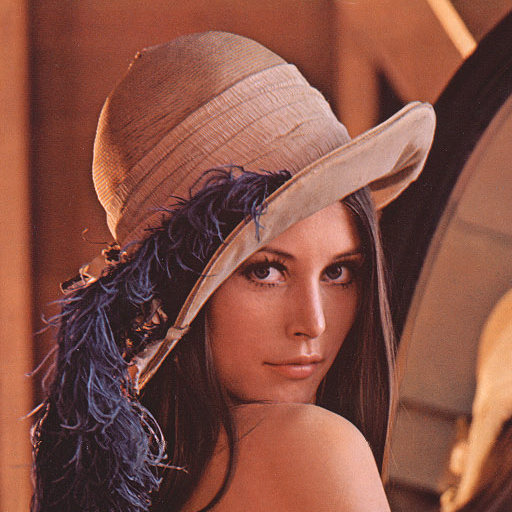
\includegraphics[width=0.2\textwidth]{imagenes/lena.png} &
   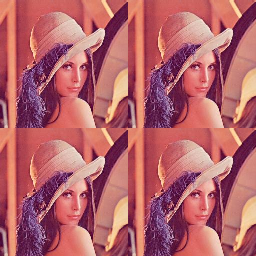
\includegraphics[width=0.2\textwidth]{imagenes/lena-smalltiles.png} &
   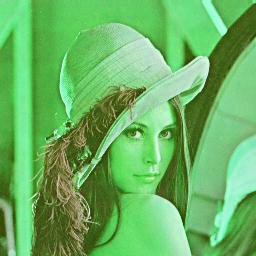
\includegraphics[width=0.2\textwidth]{imagenes/lena-rotar-canales.png} \\
   Imagen original & Smalltiles & Rotar \\
   \\
   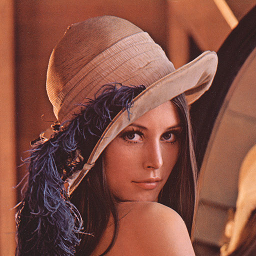
\includegraphics[width=0.2\textwidth]{imagenes/lena-pixelar.png} &
   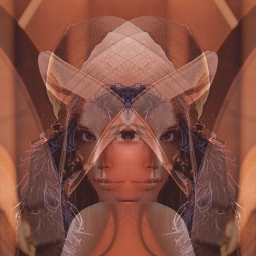
\includegraphics[width=0.2\textwidth]{imagenes/lena-combinar.png} &
   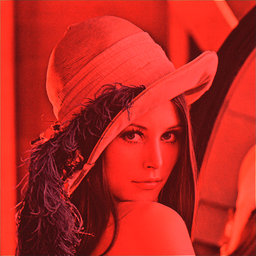
\includegraphics[width=0.2\textwidth]{imagenes/lena-colorizar.png} \\
   Pixelar & Combinar & Colorizar \\
 \end{tabular}
\end{center}

\subsection{Preliminares}

Consideramos a una imagen como una matriz de píxeles. Cada píxel está determinado por cuatro componentes: los colores azul (\Blue), verde (\Green) y rojo (\Red), y la transparencia (\Alpha). En nuestro caso particular cada una de estas componentes tendrá 8 bits (1 byte) de profundidad, es decir que estarán representadas por números enteros en el rango $[0,256)$.

% La cátedra provee una librería de funciones para cargar a memoria imágenes en formato BMP, de manera tal que su tarea se reduce a escribir funciones que trabajan con matrices de píxeles. (Detalles en sección~\ref{sec:

% Para la descripción de los filtros asumiremos una imagen de entrada $M$ de tamaño $m$ filas y $n$ columnas.

Dada una imagen $I$, notaremos $\mathsf{I}_{i,j}^k$ al valor de la componente $k \in \{ \Red, \Green, \Blue, \Alpha \}$ del píxel en la fila $i$ y la columna $j$ de la imagen.
La fila 0 corresponde a la fila de más abajo de la imagen.
La columna 0 a la de más a la izquierda.

Llamaremos $\mathsf{O}$ a la imagen de salida generada por cada filtro. Por ejemplo, el filtro identidad estaría caracterizado por la fórmula
\[ \forall k \in \{\Red,\Green,\Blue,\Alpha\} \quad \mathsf{O}_{i,j}^k = \mathsf{I}_{i,j}^k. \]

\subsection{Smalltiles}

Esta operaci\'on consiste en repetir la imagen original 4 veces, de forma m\'as chica en la imagen destino. 
Es decir, que si originalmente se tiene una imagen de tama\~no $w$ x $h$, en el destino se tendr\'an 4 im\'agenes 
de tama\~no $w/2$ x $h/2$, una en cada cuadrante. \\

% pegar una imagen de ejemplo.

Para copiar los p\'ixeles, a cada $(i, j)$ de la primera imagen destino, le corresponde el valor de la posici\'on $(2i, 2j)$ en la imagen fuente.\\

%Nota: En el caso que la entrada sea una imagen impar se debe duplicar la linea que sobra en su extremo derecho e inferior según corresponda.

\subsubsection*{Implementación y uso}

\noindent Funciones: \code{smalltiles_c}, \code{smalltiles_asm} 

\noindent Parámetros: ninguno

\subsection{Rotar canales}

Consiste en rotar los canales de color entre sí, de la siguiente manera:
\begin{center}
\textbf{R} $\longrightarrow$ \textbf{G}\\
\textbf{G} $\longrightarrow$ \textbf{B}\\
\textbf{B} $\longrightarrow$ \textbf{R}\\
\end{center}

\noindent Funciones: \code{rotar_c}, \code{rotar_asm}  

\noindent Parámetros: ninguno


\subsection{Pixelar}

El proceso de pixelar la imagen consiste en partir la imagen original en 
bloques de $2\times2$ píxeles. Por cada componente por separado, y para cada bloque de la imagen original, se genera 
un bloque del mismo tama\~no en la imagen destino y a cada uno de sus píxeles se
le asigna el promedio de los valores de los píxeles del bloque de la imagen 
original.\\

\begin{framed}
  \noindent \textbf{Nota}: El tama\~no (tanto alto como ancho) de la imagen 
  destino es m'ultiplo de $4$.
\end{framed}

\subsubsection*{Implementación y uso}

\noindent Funciones: \code{pixelar_c}, \code{pixelar_asm}

\noindent Parámetros: ninguno

\subsection{Combinar}

Dadas 2 im'agenes de igual tama\~no, este procedimiento genera una tercera 
formada a partir de estas 2. Cada píxel de la imagen resultante se forma de la 
siguiente manera:

\begin{center}
  $ I_{dst}(i,j) =  \frac{alpha \cdot (I_{src_{a}}(i,j) - 
    I_{src_{b}}(i,j))}{255.0} + I_{src_{b}}(i,j) $
\end{center}

donde $alpha \in [0.0; 255.0]$.\\

\begin{framed}
  \noindent \textbf{Nota}: Por simplicidad, este proceso se realiza con la 
  imagen original y su reflejo vertical.
\end{framed}

\subsubsection*{Implementación y uso}

\noindent Funciones: \code{combinar_c}, \code{combinar_asm},

\noindent Parámetros: 

\begin{enumerate}[-]
\item \code{alpha}: Número en punto flotante entre 0.0 y 255.0
\end{enumerate}

\noindent Ejemplo de uso: \code{combinar -i c lena.bmp}

\subsection{Colorizar}

Dada una imagen de entrada, la imagen resultado se forma en base a las
siguientes definiciones:

\begin{center}
\begin{displaymath}
\begin{array}{ccccccc}
    max_*(i, j) = max(      & I_{src\_*}(i-1, j-1) & , & I_{src\_*}(i-1, j) & , & I_{src\_*}(i-1, j+1), \\
      & I_{src\_*}(i  , j-1) & , & I_{src\_*}(i  , j) & , & I_{src\_*}(i  , j+1), \\
      & I_{src\_*}(i+1, j-1) & , & I_{src\_*}(i+1, j) & , & I_{src\_*}(i+1, j+1))
\end{array}
\end{displaymath}
\end{center}

donde $* \in \{R, G, B\}$. Luego
\begin{center}
\begin{displaymath}
 \phi_R(i, j) = \left\{
\begin{array}{l l}
  		(1 + \alpha) & \text{si $max_R(i,j) \geq max_G(i,j)$ y $max_R(i,j) \geq max_B(i,j)$}\\
  		(1 - \alpha) & \text{si no}
\end{array}
\right.
\end{displaymath}
\begin{displaymath}
 \phi_G(i, j) = \left\{
\begin{array}{l l}
  		(1 + \alpha) & \text{si $max_R(i,j) < max_G(i,j)$ y $max_G(i,j) \geq max_B(i,j)$}\\
  		(1 - \alpha) & \text{si no}
\end{array}
\right.
\end{displaymath}
\begin{displaymath}
\phi_B(i, j) = \left\{
\begin{array}{l l}
  		(1 + \alpha) & \text{si $max_R(i,j) < max_B(i,j)$ y $max_G(i,j) < max_B(i,j)$}\\
  		(1 - \alpha) & \text{si no}
\end{array}
\right.
\end{displaymath}
\end{center}

donde $0 \leq \alpha \leq 1$.

\begin{center}
\begin{displaymath}
\begin{array}{r l}
  I_{dst_R}(i, j) = &min(255, \phi_R * I_{src_R}(i, j))\\
  I_{dst_G}(i, j) = &min(255, \phi_G * I_{src_G}(i, j))\\
  I_{dst_B}(i, j) = &min(255, \phi_B * I_{src_B}(i, j))
\end{array}
\end{displaymath}
\end{center}


\begin{framed}
  \noindent \textbf{Nota}: La primera y 'ultima fila de la imagen original no
  debe ser procesada. Lo mismo sucede para la primera y 'ultima columna.
\end{framed}


\subsubsection*{Implementación y uso}

\noindent Funciones: \code{colorizar_c}, \code{colorizar_asm}

\noindent Parámetros: 

\begin{enumerate}[-]
\item \code{float alpha}: número entre 0 y 1 que define intensidad de la colorización
\end{enumerate}

% -----------------------------------------------------------------
% -----------------------------------------------------------------



% ------------------------------------------------------------------
% ------------------------------------------------------------------

%\newpage
\section{Implementación}

Para facilitar el desarrollo del trabajo práctico se cuenta con un
\emph{framework} que provee todo lo necesario para poder leer y
escribir imágenes, así como también compilar y probar las funciones
que vayan a implementar.

\subsection{Archivos y uso}

\vspace*{0.3cm}
Dentro de los archivos presentados deben completar el código de las funciones
pedidas. Puntualmente encontrarán el programa principal (de línea de
comandos), denominado \textbf{tp2}, que se ocupa de parsear las opciones
ingresadas por el usuario y ejecutar el filtro seleccionado sobre la imagen
ingresada.

\vspace*{0.3cm}
\noindent Los archivos entregados están organizados en las siguientes carpetas:

\begin{itemize}
    \itemsep0em
    \item
        \code{documentos}: Contiene este enunciado y un \emph{template}
        de informe en \LaTeX.

	\item
		\code{codigo}: Contiene el código fuente, junto con el framework
		de ejecución y testeo.
		Contiene los fuentes del programa principal,
    		junto con el \textbf{Makefile} que permite compilarlo.
		Además contiene los siguientes subdirectorios:
		\begin{itemize}
		\item
			\code{build}: Contiene los archivos objeto y ejecutables
			del TP.

		\item
			\code{filtros}: Contiene las implementaciones de los filtros

		\item
			\code{helper}: Contiene los fuentes de la biblioteca BMP y
			de la herramienta de comparación de imágenes.

		\item
			\code{img}: Algunas imágenes de prueba.

    		\item
			\code{test}: Contiene scripts para realizar tests sobre los
	        filtros y uso de la memoria.
	\end{itemize}
\end{itemize}

\subsubsection*{Compilación}

Ejecutar \texttt{make} desde la carpeta \texttt{codigo}.
Recordar que cada directorio tiene su propio \code{Makefile},
por lo que si se desea cambiar las opciones de compilación
debe buscarse el \code{Makefile} correspondiente.

\subsubsection*{Uso}
% -----------------------------------------------------------------------------

\vspace*{0.2cm}
\noindent El uso del programa principal es el siguiente:
\vspace*{-0.2cm}
\begin{itemize}
    \item [\code{\$}]
        \code{./tp2 $<$opciones$>$ $<$nombre\_filtro$>$
              $<$nombre\_archivo\_entrada$>$ [parámetros...]}
\end{itemize}


Los filtros que se pueden aplicar y sus parámetros son
los especificados en la sección filtros, apartado
``Implementación y uso``


Las opciones que acepta el programa son las siguientes:
\begin{itemize}
  \itemsep0em
  \item \code{-h, --help} \\
  \indent Imprime la ayuda

  \item \code{-i, --implementacion NOMBRE\_MODO} \\
  \indent Implementación sobre la que se ejecutará el proceso
    seleccionado. Los implementaciones disponibles son: c, asm

  \item \code{-t, --tiempo CANT\_ITERACIONES} \\
  \indent Mide el tiempo que tarda en ejecutar el filtro sobre la
    imagen de entrada una cantidad de veces igual a CANT\_ITERACIONES

%  \item \code{-f, --frames} \\
%  \indent Genera frames independientes
%    en vez de armar un archivo de video. Es utilizado para testing. Sólo para archivos de video.

  \item \code{-o, --output DIRECTORIO} \\
  \indent Genera el resultado en DIRECTORIO.
    De no incluirse, el resultado se guarda en el mismo directorio
    que el archivo fuente

  \item \code{-v, --verbose} \\
  \indent Imprime información adicional

%  \item \code{-w, --video} \\
%  \indent Interpreta el archivo de entrada como video.
%    En caso de no estar, se interpreta la entrada como una imagen.

\end{itemize}

\vspace*{0.3cm}
\noindent Por ejemplo:
\vspace*{-0.2cm}
\begin{itemize}
    \item [\code{\$}]
        \code{./tp2 -v colorizar -i asm lena.bmp 0.4}
\end{itemize}

\noindent Aplica el filtro de \textbf{colorizar} al archivo lena.bmp
utilizando la implementación en lenguaje asm del filtro, pasándole como parámetro 0.4 como valor de alpha.

\subsection{Código de los filtros}

Para implementar los filtros descriptos anteriormente, tanto en C como
en ASM se deberán implementar las funciones especificadas en la sección
\ref{filtros}.
Las imágenes se almacenan en memoria en color, en el orden
B (blue), G (green), R (red), A (alpha).

% -----------------------------------------------------------------------------
Los parámetros genéricos de las funciones son:
\begin{itemize}
  \itemsep0em
  \item[-]
      \code{src}\rmfamily: Es el puntero al inicio de la matriz de
      elementos de 32 bits sin signo (el primer byte corresponde al canal azul
      de la imagen (B), el segundo el verde (G), el tercero el rojo (R)), y el
      cuarto el alpha (A) que
      representa a la imagen de entrada. Es decir, como la imagen está en
      color, cada píxel está compuesto por 4 bytes.

   \item[-]
      \code{dst}\rmfamily: Es el puntero al inicio de la matriz de
      elementos de 32 bits sin signo que representa a la imagen de salida.

   \item[-]
      \code{filas}\rmfamily: Representa el alto en píxeles de la imagen, es
      decir, la cantidad de filas de las matrices de entrada y salida.

   \item[-]
      \code{cols}\rmfamily: Representa el ancho en píxeles de la imagen, es
      decir, la cantidad de columnas de las matrices de entrada y salida.

   \item[-]
      \code{src\_row\_size}\rmfamily: Representa el ancho en bytes de cada fila
      de la imagen incluyendo el padding en caso de que hubiere. Es decir, la cantidad de bytes que hay que avanzar para moverse a la misma columna de fila siguiente/anterior.
\end{itemize}

% --------------------------------------------------------------------
% --------------------------------------------------------------------

%\newpage
\subsubsection*{Consideraciones}

Las funciones a implementar en lenguaje ensamblador deben utilizar el set de
instrucciones \textbf{SSE}, a fin de optimizar la performance de las mismas.
Tener en cuenta lo siguiente:

\begin{itemize}
  \itemsep0em
  \item El ancho de las imágenes es siempre mayor a 16 píxeles.

  \item No se debe perder precisión en ninguno de los cálculos, a menos que se indique lo contrario.

  \item La implementación de cada filtro deberá estar optimizada para el
    filtro que se está implementando. No se puede hacer una función que
    aplique un filtro genérico y después usarla para implementar los que se
    piden.

  \item Para el caso de las funciones implementadas en lenguaje ensamblador,
    deberán trabajar con \textbf{al menos 2 píxeles simultámeamente}.

    De no ser posible esto para algún filtro, deberá justificarse
    debidamente en el informe.

  \item El procesamiento de los píxeles se deberá hacer
    \textbf{exclusivamente} con instrucciones \textbf{SSE}.
    No está permitido procesarlos con registros de propósito general,
    salvo para tratatimiento de casos borde. En tal caso se deberá
    justificarse debidamente y hacer un análisis del costo computacional.

  \item El TP se tiene que poder ejecutar en las máquinas del laboratorio.
\end{itemize}



\subsection{Formato BMP}

El formato BMP es uno de los formatos de imágenes mas simples: tiene un encabezado y un mapa de bits que representa la información de los pixeles.
En este trabajo práctico se utilizará una biblioteca provista por la cátedra para operar con archivos en ese formato.
Si bien esta biblioteca no permite operar con archivos con paleta, es posible leer tres tipos de formatos, tanto con o sin transparencia.
Ambos formatos corresponden a los tipos de encabezado: BITMAPINFOHEADER (40 bytes), BITMAPV3INFOHEADER (56 bytes) y BITMAPV5HEADER (124 bytes).
\smallskip

El código fuente de la biblioteca está disponible como parte del material, deben seguirlo y entenderlo.
Las funciones que deben implementar reciben como entrada un puntero a la imagen. Este puntero corresponde al mapa de bits almacenado en el archivo.
El mismo está almacenado de forma particular: \textbf{las líneas de la imagen se encuentran almacenadas de forma invertida}.
Es decir, en la primera fila de la matriz se encuentra la última línea de la imagen, en la segunda fila se encuentra la anteúltima y así sucesivamente.
Dentro de cada línea los pixeles se almacenan de izquierda a derecha, y cada pixel \textbf{en memoria se guarda en el siguiente orden: B, G, R, A}.



% -----------------------------------------------------------------
% -----------------------------------------------------------------

\subsection{Herramientas y tests}

En el código provisto, podrán encontrar varias herramientas
que permiten verificar si los filtros funcionan correctamente.

\subsubsection*{Diff}
La herramienta \code{diff} permite comparar dos imágenes.
El código de la misma se encuentra en \texttt{helper}, y se
compila junto con el resto del trabajo práctico.
El ejecutable, una vez compilado, se almacenará en
\texttt{build/bmpdiff}.
La aplicación se utiliza desde linea de comandos de la forma:

\begin{codesnippet}
./build/bmpdiff $<$opciones$>$ $<$archivo_1$>$ $<$archivo_2$>$ $<$epsilon$>$
\end{codesnippet}


Esto compara los dos archivos según las componentes de cada pixel, siendo epsilon la diferencia máxima permitida entre pixeles correspondientes de las dos imágenes.
Tiene dos opciones: listar las diferencias o generar imágenes blanco y negro por cada componente, donde blanco es marca que hay diferencia y negro que no.

\bigskip
Las opciones soportadas por el programa son:

\begin{tabular}{l|l}
  \verb|-i|, \verb|--image|    &  Genera imágenes de diferencias por cada componente.\\
  \verb|-v|, \verb|--verbose|  &  Lista las diferencias de cada componente y su posición en la imagen.\\
  \verb|-a|, \verb|--value|    &  Genera las imágenes mostrando el valor de la diferencia.\\
  \verb|-s|, \verb|--summary|  &  Muestra un resumen de diferencias.\\
\end{tabular}

\subsubsection*{Tests}
Para verificar el correcto funcionamiento de los filtros,
además del comparador de imágenes, se provee un binario
con la solución de la cátedra y varios scripts de test.
El binario de la cátedra se encuentra en la carpeta {\code{codigo/build}}.
El comparador de imágenes se ubica en la carpeta {\code{codigo/helper}}, y debe
compilarse antes de correr los scripts (correr {\code{make}} en la carpeta {\code{codigo/helper}}).

Los scripts de test toman como entrada las corridas especificadas en {\code{corridas.txt}}.
Para cada imagen de test, se ejecutan todas las corridas ahí indicadas.
Para verificar que la implementación funciona correctamente con imágenes de distinto
tamaño,{ \code{generar\_imagenes.sh}} genera variaciones de las imágenes fuente
(que se encuentran en {\code{codigo/tests/data}}), y las deposita en {\code{imagenes\_a\_testear}}.
Para que este script funcione correctamente se requiere la utilidad {\code{convert}} que se encuentra
en la biblioteca {\code{imagemagick}}.\footnote{Para instalar \code{sudo apt-get install imagemagick}}.

El archivo {\code{test\_dif\_cat.sh}} verifica que los resultados de la catedra den igual que la implementación de C.
{\code{test\_dif\_c\_asm.sh}} verifica que los resultados de las versiones de C y Assembler sean iguales.
{\code{test\_mem.sh}} chequea que no haya problemas en el uso de la memoria.
Finalmente, {\code{test\_all.sh}} corre todos los checks anteriores uno después del otro.

\subsection{Mediciones de rendimiento}

La forma de medir el rendimiento de nuestras implementaciones se realizará por medio de la toma de tiempos de ejecución.
Como los tiempos de ejecución son muy pequeños, se utilizará uno de los contadores de performance que posee el procesador.

La instrucción de assembler \texttt{rdtsc} permite obtener el valor del Time Stamp Counter (TSC) del procesador.
Este registro se incrementa en uno con cada ciclo del procesador.
Obteniendo la diferencia entre los contadores antes y después de la llamada a la función, podemos obtener la cantidad de ciclos de esa ejecución.
Esta cantidad de ciclos no es siempre igual entre invocaciones de la función, ya que este registro es global del procesador y se ve afectado por una serie de factores.

Existen principalmente distintas problemáticas a solucionar:

\begin{enumerate}
 \item La ejecución puede ser interrumpida por el \emph{scheduler} para realizar un cambio de contexto, esto implicará contar muchos más ciclos (\emph{outliers}) que si nuestra función se ejecutara sin interrupciones.
 \item Los procesadores modernos varían su frecuencia de reloj, por lo que la forma de medir ciclos cambiará dependiendo del estado del procesador.
 \item El comienzo y fin de la medición deben realizarse con la suficiente
 exactitud como para que se mida solamente la ejecución de los filtros, sin
 ser afectada por ruidos como la carga o el guardado de las imágenes.
\end{enumerate}

Para medir tiempos deberán idear e implementar una metodología que les permita evitar estos tres problemas.
En el archivo \texttt{tp2.c} se provee código para realizar una
medición de tiempo básica. El mismo podrá ser modificado para
mejorar y automatizar las mediciones.
Se recomienda utilizar un framework de medición automatizado
como \code{metrika}\footnote{pip3 install --user metrika |
\url{https://github.com/dc-uba/metrika}}
para evitar errores de medición sistemáticos, es decir, aquellos
causados por una incorrecta ejecucción de las mediciones.



% ---------------------------------------------------------------------
% ---------------------------------------------------------------------


\section{Ejercicios}

Se deberá implementar el código de los filtros, realizar
un análisis de su performance y presentar un informe de los
resultados.

\subsection{Implementación}

Deberán implementar (al menos) una versión de cada filtro en C y otra en lenguaje ensamblador, utilizando instrucciones SSE.
La implementación inicial de los filtros que sólo realicen cálculos
con números enteros no deberá perder precisión. Es posible que se
desee realizar optimizaciones al costo de perder algo de precisión.
Esto será aceptable siempre y cuando se analice también la calidad
de la imagen resultante en la versión optimizada contra la no
optimizada.

\subsection{Análisis}

Las siguientes preguntas deben ser usadas como guía.
La evaluación del trabajo práctico no sólo consiste en responder
las preguntas, sino en desarrollar y responder nuevas preguntas
sugeridas por ustedes mismos buscando entender y razonar sobre
el modelo de programación SIMD y la microarquitectura del procesador.


\begin{itemize}
\item ¿Cuál implementación es ``mejor''?
\item ¿Qué métricas se pueden utilizar para calificar las implementaciones y cuantificarlas?
\item ¿En qué casos? ¿De qué depende? ¿Depende del tamaño de la imagen? ¿Depende de la imagen en sí? ¿De los parámetros?
\item ¿Cómo se podrían mejorar las métricas de las implementaciones propuestas? ¿Cuáles no se pueden mejorar?
\item ¿Es una comparación justa? ¿De qué depende la velocidad del
código C? ¿Cómo puede optimizarse?
\item ¿Cuál es la cantidad de instrucciones ejecutadas por pixel en cada implementación? ¿Y de accesos a memoria? ¿Se condice empíricamente esta diferencia en la performance de los filtros?
\item ¿Hay diferencias en operar con enteros o punto flotante? ¿La imagen final tiene diferencias significativas?
\item ¿El overhead de llamados a funciones es significativo? ¿Se puede medir?
\item ¿Las limitaciones de performance son causadas por los accesos a memoria?, ¿o a la memoria cache?, ¿esta se podría acceder mejor?
\item ¿Y los saltos condicionales? ¿Afectan la performance? ¿Es posible evitarlos total o parcialmente?
\item ¿El patrón de acceso a la memoria es desalineado? ¿Hay forma de mejorarlo? ¿Es posible medir cuánto se pierde?
\end{itemize}


\subsection{Informe}

El informe debe incluir las siguientes secciones:

\begin{enumerate}
    \item
        \textbf{Carátula} Contiene

        \begin{itemize}
            \item número / nombre del grupo
            \item nombre y apellido de cada integrante
            \item número de libreta y mail de cada integrante
        \end{itemize}

    \item
        \textbf{Introducción}
        Describe lo realizado en el trabajo práctico.

    \item
        \textbf{Desarrollo}\\
        Describe cada una de las funciones que implementaron.
	    Para la descripción de cada función deberán decir cómo
        opera una iteración del ciclo de la función.
        Es decir, cómo mueven los datos a los registros, cómo los
        reordenan para procesarlos, las operaciones que se aplican
        a los datos, etc.
        Además se agregará un detalle más profundo de las secciones
        de código que consideren más importantes.
        Para esto pueden utilizar pseudocódigo, diagramas (mostrando
        gráficamente el contenido de los registros \texttt{XMM}) o
        cualquier otro recurso que le sea útil para describir la
        adaptación del algoritmo al procesamiento simultáneo SIMD.
        No se deberá incluir el código assembler de las funciones
        (aunque se pueden incluir extractos en donde haga falta).

	\item
		\textbf{Resultados}\\
		Deberán \textbf{analizar} y \textbf{comparar} las
		implementaciones de las funciones en su versión \textbf{C}
		y \textbf{assembler} y mostrar los resultados obtenidos a
		través de tablas y gráficos.
		Para esto deberán plantear experimentos que les permitan
		comprobar las diferencias de performance e hipotetizar
		sobre sus causas.

		Deberán además explicar detalladamente los resultados
		obtenidos y analizarlos.
		En el caso de encontrar anomalías o comportamientos no
		esperados deberán construir nuevos experimentos para
		entender qué es lo que sucede.


	    Utilizar como guía para la realización de experimentos
	    las preguntas de la sección anterior.
	    Al responder estas preguntas (y otras que vayan surgiendo),
	    se deberán analizar y comparar
        las implementaciones de cada funcion en su versión
        \texttt{C} y \texttt{ASM}, mostrando los resultados obtenidos
        a través de tablas y gráficos.
        También se deberá \emph{comentar} los resultados obtenidos.
	    %En el caso de que sucediera que la versión en C anduviese más
        %rápidamente que su versión ASM, \textbf{justificar
        %fuertemente} a qué se debe esto.

    \item
        \textbf{Conclusión}
        Reflexión final sobre los alcances del trabajo práctico,
        la programación vectorial a bajo nivel,
        problemáticas encontradas, y todo lo que consideren pertinente.
\end{enumerate}

%El informe no puede exceder las \textbf{20} páginas, sin contar la
%carátula.

\vspace*{0.3cm}
\textbf{Importante}: El informe se evalúa de manera independiente del
código.
Puede reprobarse el informe, y en tal caso deberá ser reentregado para
aprobar el trabajo práctico.


% --------------------------------------------------------------------
% --------------------------------------------------------------------

\section{Entrega y condiciones de aprobación}

El presente trabajo es de carácter \textbf{grupal}, siendo los grupos de
\textbf{3 personas}, pudiendo ser de 2 personas en casos excepcionales previa
consulta y confirmación del cuerpo docente. Se deberá entregar un archivo
comprimido con el mismo contenido que el dado para realizarlo, habiendo
modificado sólo los archivos que tienen como nombre las funciones a
implementar. \textbf{No} debe incluírse ningún tipo de archivo binario extra
como código objeto o ejecutables.\\

%\textbf{Es codición necesaria para la aprobación de este trabajo que pasen correctamente
%todos los tests de la catedra.}

La fecha de entrega última de este trabajo es \textbf{Martes 27 de Septiembre} y deberá
ser entregado a través de la página web. El sistema s\'olo aceptará entregas
de trabajos hasta las \textbf{17:00hs} del día de entrega. La fecha límite para la \textbf{reentrega} es el día \textbf{Martes 1 de Noviembre}\\

Ante cualquier problema con la entrega, comunicarse por
mail a la \textbf{lista de docentes}.\\

\end{document}



\newpage

\subsection{Pixelar}
\subsubsection{Implementación}
Como el filtro necesita la información de dos filas para realizar el promedio, recorro tanto la imagen fuente como la imagen destino con dos punteros. Estos se mueven de forma paralela, es decir, en las mismas columnas pero en filas consecutivas. Al trabajar de esta forma y utilizando instrucciones SIMD podemos aplicar los cambios a ocho píxeles a la vez (cuatro por punteros).
\\Para no perder precisión todas las operaciones que se necesitan para obtener los promedios se realizan en enteros. Una vez calculados (uno por grupo de 4 píxeles) se remplazan en la imagen destino los valores originales de los píxeles por el valor promedio correspondiente.
\\Se itera sobre la imagen columna por columna, y, una vez que se terminaron de recorrer las dos filas paralelas, se decrementa el contador que contiene la mitad de la cantidad total de filas a recorrer. De esta manera, una vez que dicho contador llegó a cero, se terminó de recorrer la imagen. Como se opera de a 4 píxeles por puntero, se divide la cantidad de columnas (que están en píxeles) por cuatro y los punteros avanzan de a 16 bytes. A su vez, cuando se terminan de recorrer las filas, los punteros avanzan, la cantidad de columnas por cuatro bytes, saltándose cada puntero una fila. No se puede operar de a más píxeles por vez porque cada uno ocupa 32 bits, entonces solo se pueden almacenar cuatro de ellos por vez en los registros de SIMD.
\\
\\
La implementación realizada en C itera sobre la imagen con dos ciclos anidados (avanzando por columnas), de a 4 píxeles por vez, avanzando de a dos columnas y dos filas a la vez. Simplemente se calcula el promedio en cuatro píxeles y se coloca este valor en la imagen destino en las posiciones de los píxeles procesados. Si bien las cuentas se realizan de manera muy similar a la implementación en lenguaje ensamblador, esta última recorre la imagen más rápido al procesar de a 8 píxeles por iteración, por lo que el rendimiento debería ser mayor.


\newpage

\end{document}


